% Copyright 2026 Sreeram Anil
% SPDX-License-Identifier: CC-BY-4.0
% =============================================================================
%  Unknown-input observer
% =============================================================================
\chapter{Unknown-Input Observer (UIO)}
\label{ch:uio}

\section*{At a glance}
\begin{tabular}{@{}l>{\raggedright\arraybackslash}p{0.76\textwidth}@{}}
Family & Deterministic observers \\
Header & \texttt{include/estkit/observers/uio.hpp} \\
Registered name & \texttt{UIO} \\
State dimension & $n_x = 4$ plus an $n_x$-dimensional internal state $\vz$; $n_y = 1$ \\
Cost per step & $\mathcal{O}(n_x^2)$ steady state; $\approx 0.6\,\mu$s/step measured \\
Primary references & \cite{chen1996uio,chenpatton1999,darouach1994uio,houmuller1992uio,zhao2017observability} \\
\end{tabular}

\section{Motivation and aerospace/BMS relevance}
The disturbance observers of \Cref{ch:eso,ch:dob} \emph{estimate} the unknown input and subtract
it.  The unknown-input observer does something stronger: it makes the estimation error
\emph{algebraically independent} of the unknown input, whatever that input does.  No bound on its
magnitude, no assumption that it is slow, no random-walk model --- the decoupling is exact
\cite{chen1996uio,chenpatton1999}.

For a battery the unknown input of interest is the current-sensor error, and the reason exact
decoupling is attractive is that a real current-sensor fault is not a random walk.  A Hall-effect
sensor exposed to a stray field from an adjacent bus bar produces an offset that steps with the
motor current; a shunt with a degraded thermal path produces one that follows the pack
temperature.  A structure whose SOC estimate is provably insensitive to \emph{any} such signal is
worth more in a safety case than one whose performance depends on the disturbance being slow.

The price is also structural and is the interesting part of this chapter: the decoupling consumes
one degree of freedom of the observer, and the modes it gives up --- the invariant zeros of the
triple $(\mA,\bm{E},\mC)$ --- cannot be moved.  The design is therefore a genuine trade between
disturbance rejection and bandwidth, and this benchmark quantifies it.

\section{Problem statement and assumptions}
The measured input is corrupted on one channel, $\vu^{\mathrm{true}} = \vu - d\,\bm{e}_j$, with
$d$ arbitrary and unknown.  Linearising, the plant is
\begin{equation}
\vx_{k+1} = f(\vx_k,\vu_k) + \bm{E}\,d_k , \qquad
\bm{E} \triangleq -\frac{\partial f}{\partial u_j} , \qquad
y_k = h(\vx_k,\vu_k) + v_k .
\label{eq:uio-plant}
\end{equation}
\begin{assumption}[Matching / rank condition]\label{as:uio-rank}
$\operatorname{rank}(\mC\bm{E}) = \operatorname{rank}(\bm{E})$.
\end{assumption}
\begin{assumption}[Detectability of the decoupled pair]\label{as:uio-det}
$(\bm{T}\mA,\mC)$ is detectable, with $\bm{T}$ defined in \eqref{eq:uio-TH}.  Equivalently, the triple
$(\mA,\bm{E},\mC)$ has no invariant zero on or outside the unit circle
\cite[Ch.~3]{chenpatton1999}.
\end{assumption}

\section{Derivation}

\subsection{The Chen--Patton--Zhang construction}
Set
\begin{equation}
\mH = \bm{E}\,(\mC\bm{E})^{+} , \qquad \bm{T} = \mI - \mH\mC ,
\label{eq:uio-TH}
\end{equation}
where $(\cdot)^+$ is the Moore--Penrose pseudo-inverse (a scalar reciprocal when $n_y=1$ and
$\bm{E}$ has one column).  Then
\begin{equation}
\bm{T}\bm{E} = \bm{E} - \bm{E}(\mC\bm{E})^{+}(\mC\bm{E}) = \bm{0}
\label{eq:uio-TE}
\end{equation}
under \Cref{as:uio-rank}: $\bm{T}$ annihilates the disturbance direction.  Choose $\mK_1$ and set
\begin{equation}
\mF = \bm{T}\mA - \mK_1\mC , \qquad \mK = \mK_1 + \mF\mH ,
\label{eq:uio-FK}
\end{equation}
and run
\begin{equation}
\vz_{k+1} = \mF\vz_k + \bm{T}\mB\vu_k + \mK\vy_k , \qquad
\xhat_k = \vz_k + \mH\vy_k .
\label{eq:uio-rec}
\end{equation}

\begin{theorem}[Exact decoupling, \cite{chen1996uio}]\label{th:uio}
With \eqref{eq:uio-TH}--\eqref{eq:uio-rec} the estimation error
$\veps_k = \vx_k - \xhat_k$ obeys $\veps_{k+1} = \mF\veps_k$ exactly, independently of $d$.
\end{theorem}
\begin{proof}[Proof sketch]
$\veps_{k+1} = \vx_{k+1} - \vz_{k+1} - \mH\vy_{k+1}
= (\mI-\mH\mC)\vx_{k+1} - \mF\vz_k - \bm{T}\mB\vu_k - \mK\vy_k
= \bm{T}(\mA\vx_k + \mB\vu_k + \bm{E} d_k) - \mF\vz_k - \bm{T}\mB\vu_k - \mK\mC\vx_k$.
The $\bm{E} d_k$ term vanishes by \eqref{eq:uio-TE}.  Substituting
$\vz_k = \xhat_k - \mH\mC\vx_k$ and using $\mK = \mK_1+\mF\mH$ gives
$\veps_{k+1} = (\bm{T}\mA-\mK_1\mC)\vx_k - \mF\xhat_k = \mF\veps_k$.
\end{proof}

\subsection{Fixed modes: the price of decoupling}
\label{sec:uio-zeros}
$\bm{T}$ has rank $n_x - \operatorname{rank}(\bm{E})$ because $\bm{T}\bm{E}=\bm{0}$, so $\bm{T}\mA$ is singular
and $(\bm{T}\mA,\mC)$ can only be \emph{detectable}, not observable, in general.  The modes that
$\mK_1$ cannot move are exactly the invariant zeros of $(\mA,\bm{E},\mC)$, i.e. the $z$ for which
\begin{equation}
\operatorname{rank}\begin{bmatrix} z\mI-\mA & -\bm{E}\\ \mC & 0\end{bmatrix} < n_x + \operatorname{rank}(\bm{E}) .
\label{eq:uio-zeros}
\end{equation}
For the cell model at $25^\circ$C, $\soc=0.5$ the numerically computed spectral radius of $\mF$ is
$0.99973$ for \emph{every} $\mK_1$ tried, from an LQE design with $\mQ$ scaled over four orders of
magnitude --- an unambiguous experimental confirmation that this mode is fixed.  It corresponds to
a $375$\,s time constant, and it is the bandwidth the observer pays for exactness.  This is the
central design trade of the method and it is visible directly in the benchmark's
\texttt{init\_error} column.

\subsection{Design of the proportional gain}
$\mK_1$ is a \emph{prediction}-form gain ($\mF = \bm{T}\mA-\mK_1\mC$), so no $\mA\inv$ conversion is
applied.  Two designs are offered.  Pole placement on $(\bm{T}\mA,\mC)$ is available but is not the
default: the observability matrix of the decoupled pair is far worse conditioned than that of the
original pair ($\det\mathcal{O}_{\bm{T}\mA}\approx-9\times10^{-60}$ for the cell), and even with the
shift-and-scale of \Cref{sec:lue-cond} the assignment of a mode that is structurally fixed is
ill-posed.  The default is therefore the LQE design: solve \eqref{eq:lue-dare} for the pair
$(\bm{T}\mA,\mC)$ and take $\mK_1 = (\bm{T}\mA)\,\mK_{\mathrm{filter}}$, the conversion from the
current-estimator gain returned by the Riccati recursion to the prediction gain needed by
\eqref{eq:uio-FK}.  The resulting $\mF$ is checked for stability before the design is accepted.

\subsection{Nonlinear realisation}
\label{sec:uio-nonlin}
The plant here is nonlinear, so \eqref{eq:uio-rec} is used with the linearisation $(\mA,\mC,\bm{E})$
at the current estimate and two substitutions:
\begin{align}
\bm{T}\mB\vu_k &\ \longrightarrow\ \bm{T}\big(f(\xhat_k,\vu_k) - \mA\xhat_k\big) ,
\label{eq:uio-sub1}\\
\vy_k &\ \longrightarrow\ \tilde{y}_k \triangleq \mC\xhat_k + \big(y_k - h(\xhat_k,\vu_k)\big) .
\label{eq:uio-sub2}
\end{align}
Substitution \eqref{eq:uio-sub1} replaces the affine input term by the affine part of the true
nonlinear prediction, and reduces to $\bm{T}\mB\vu$ exactly when $f$ is affine.  Substitution
\eqref{eq:uio-sub2} is the affine-equivalent output: it equals $y$ exactly when $h$ is affine, and
in general differs by the second-order remainder of $h$.  The approximation is therefore first
order in the estimation error; the neglected terms are $\mathcal{O}(\norm{\veps}^2)$ through the
curvature of the OCV curve, which for $|\veps_{\soc}|<0.05$ and the NMC OCV used here is below
$0.1$\,mV.  \Cref{th:uio} holds exactly for the affine part and approximately at that order.

\subsection{Direct feed-through: what is not decoupled}
\label{sec:uio-feed}
Classical UIO theory assumes $y = \mC\vx$.  A current-sensor bias, however, also changes the
terminal voltage instantaneously through the ohmic drop:
\begin{equation}
y = h(\vx, \vu - d\,\bm{e}_j) \approx \mC\vx - D_j\,d , \qquad D_j = \frac{\partial h}{\partial u_j} = -R_0 .
\label{eq:uio-D}
\end{equation}
That path is \emph{not} annihilated by $\bm{T}$, and it leaves a residual sensitivity of order
$(\mK+\mH)D_j d$ in \Cref{th:uio}.  For the cell $R_0 = 12$\,m$\Omega$, so a $0.25$\,A bias
injects $3$\,mV; with $\mH_{\soc}=0.042$ and $\mK_{\soc}=7.4\times10^{-4}$ the resulting SOC
sensitivity is of order $1.3\times10^{-4}$ per $0.25$\,A --- two orders of magnitude smaller than
the $5\times10^{-3}$ that the same bias produces in an observer without decoupling.  The
approximation is therefore benign, and the measured \texttt{current\_bias} performance confirms
it.

\subsection{Disturbance reconstruction}
From \eqref{eq:uio-plant} the one-step-ahead residual against a prediction that ignores $d$ is
$\mC\bm{E} d + v$, so
\begin{equation}
\hat{d}_k = \frac{r_k}{\mC\bm{E}} ,
\label{eq:uio-drec}
\end{equation}
low-pass filtered with time constant \texttt{d\_tau\_steps} because a single sample is pure noise.
This is exposed through \texttt{disturbance()} and is a genuine current-sensor-bias estimate, in
amperes.  It is clamped to $\pm d_{\max}$, the sensor's specified bias range, before and after
filtering; the next subsection explains why that clamp is not cosmetic.

\subsection{Conditioning of the decoupling, and graceful degradation}
\label{sec:uio-cond}
\Cref{as:uio-rank} is a rank test, but the \emph{numerical} quality of the design is governed by a
different quantity.  Because $\xhat = \vz + \mH\tilde{y}$ feeds the raw measurement into the state
along $\bm{E}$, a persistent \emph{output}-model error $\delta$ appears in the estimate multiplied
by
\begin{equation}
\norm{\mH}_\infty = \frac{\norm{\bm{E}}_\infty}{|\mC\bm{E}|} .
\label{eq:uio-cond}
\end{equation}
Exact rejection of the unknown input is therefore bought with a $1/|\mC\bm{E}|$ sensitivity to
everything else the model gets wrong, and \eqref{eq:uio-cond} is not a property of the plant alone
--- it is a property of the \emph{parameter set}.  For the cell,
$\mC\bm{E} = (\partial\ocv/\partial\soc)\bm{E}_{\soc} - \bm{E}_{v_1} - \bm{E}_{v_2} + M\bm{E}_h$,
and the two dominant terms partially cancel.  With the nominal ECM parameters the cancellation is
mild and $\norm{\mH}_\infty = 1.7$--$2.2$ across all twelve scenarios.  With the parameters
identified against the single-particle plant, whose $R_1$ is an order of magnitude smaller, the
cancellation is severe: $\mC\bm{E}$ falls from $1.31\times10^{-4}$ to $1.8\times10^{-5}$ and
$\norm{\mH}_\infty$ rises to $15$ at $25^\circ$C and $21$ at $70^\circ$C.  The structured
ECM-versus-SPM voltage error is then amplified sevenfold to tenfold, and the observer, applied
naively, produces a $10\,\%$ SOC error on the SPM \texttt{nominal} scenario and $58\,\%$ on
\texttt{hot} --- while every other observer in this family stays between $0.5$ and $1\,\%$.

The remedy is to make the decoupling \emph{partial} rather than all-or-nothing.  Replace
\eqref{eq:uio-TH} by
\begin{equation}
\mH = \theta\,\bm{E}(\mC\bm{E})^{+} , \qquad \theta\in[0,1] ,
\label{eq:uio-theta}
\end{equation}
so that $\bm{T}\bm{E} = (1-\theta)\bm{E}$: the unknown input is \emph{attenuated} by $(1-\theta)$
instead of removed, and the remainder is left to the $\mK_1$ feedback like any other disturbance.
$\theta=1$ is the exact Chen--Patton--Zhang observer; $\theta=0$ is an ordinary LQE observer in
prediction form.  The estimator therefore degrades continuously towards ``no decoupling'' instead
of failing, which is the property that was missing.

Two factors set $\theta$:
\begin{equation}
\theta = \underbrace{\min\!\Big(1,\ \frac{h_{\max}|\mC\bm{E}|}{\norm{\bm{E}}_\infty}\Big)}
         _{\text{a-priori conditioning budget}}
        \cdot
         \underbrace{\min\!\Big(1,\ \frac{d_{\max}}{\;\overline{|\hat{d}|}\;}\Big)}
         _{\text{a-posteriori admissibility}} .
\label{eq:uio-gate}
\end{equation}
The second factor is the important one and it is worth stating as a principle.  $\hat{d}$ of
\eqref{eq:uio-drec} is \emph{the unknown input that the residual implies}.  If its filtered
magnitude exceeds the physical bound $d_{\max}$, then the residual demonstrably is not an input
bias, hypothesis \eqref{eq:uio-plant} is false, and the observer must stop paying for a decoupling
it cannot use.  This is a self-test the structure supplies for free: the UIO is the only observer
in this family that computes, as a by-product, the quantity that falsifies its own modelling
assumption.  Measured at the end of a mission with $d_{\max}=5$\,A and $h_{\max}=4$: on the ECM
plant $\theta = 0.28$--$0.38$ and the reconstruction is admissible throughout, while on the SPM
plant $\theta = 0.04$--$0.05$ and the observer is effectively a plain LQE observer.  (The gate is
computed on a $300$\,s horizon, so the mission-average $\theta$ on the ECM sits below $1$ even
where the instantaneous reconstruction is small; what matters is the order-of-magnitude
separation between the two plants, which is a factor of seven.)

\subsection{Re-basing across a re-design}
One implementation consequence of \eqref{eq:uio-theta} is easy to miss and fatal if missed.  The
internal variable estimates $\bm{T}\vx = \vx - \mH\mC\vx$, so \emph{its meaning changes with}
$\mH$.  A re-design that changes $\mH$ must therefore shift $\vz$ by
$(\mH_{\text{old}} - \mH_{\text{new}})\tilde{y}$ to keep $\xhat = \vz + \mH\tilde{y}$ continuous;
without the shift, a change of $\theta$ moves the estimate by several volts times $\Delta\mH$.
The implementation computes $\tilde{y}$ before calling the scheduler for exactly this reason.

\section{Algorithm}
\begin{algorithm}[H]
\caption{UIO --- one sampling period}
\begin{algorithmic}[1]
\Require $\xhat_{k-1}$, internal state $\vz$, $\tilde{y}_{k-1}$, $\vu_{k-1}$, $y_k$, $\vu_k$
\State \textbf{Time update:} $\mA \gets \texttt{jac\_F}(\xhat_{k-1},\vu_{k-1})$; \quad $\vx_f \gets f(\xhat_{k-1},\vu_{k-1})$
\State $\vz \gets \mF\vz + \bm{T}(\vx_f - \mA\xhat_{k-1}) + \mK\tilde{y}_{k-1}$; \quad $\xhat_k \gets \vx_f$ \Comment{prior estimate for $\hat{y}$}
\State \textbf{Prior output:} $\hat{y}_k \gets h(\xhat_k,\vu_k)$; \quad $\mC\gets\texttt{jac\_H}(\xhat_k,\vu_k)$
\If{the linearisation has moved by more than $\delta_{\mathrm{tol}}$}
  \State $\bm{E} \gets -\partial f/\partial u_j$; \quad check $|\mC\bm{E}| > \epsilon_{\mathrm{rank}}\,\norm{\mC}\norm{\bm{E}}$
  \State $\mH \gets \bm{E}/(\mC\bm{E})$, \ $\bm{T} \gets \mI-\mH\mC$, \ $\mK_1 \gets$ LQE gain on $(\bm{T}\mA,\mC)$
  \State $\mF \gets \bm{T}\mA-\mK_1\mC$, \ $\mK \gets \mK_1+\mF\mH$; accept only if $\rho(\mF)<1$
\EndIf
\State $r_k \gets y_k - \hat{y}_k$; \quad $\tilde{y}_k \gets \mC\xhat_k + r_k$
\State $\xhat_k \gets \vz + \mH\tilde{y}_k$; \quad $\xhat_k \gets \operatorname{constrain}(\xhat_k)$
\State $\hat{d} \gets a\hat{d} + (1-a)\,r_k/(\mC\bm{E})$
\Ensure $\xhat_k$, $\hat{d}$
\end{algorithmic}
\end{algorithm}
At the first update $\vz$ is initialised as $\xhat_0 - \mH\tilde{y}_0$ so that the estimate does
not jump.  If the rank condition fails, $\mH = \bm{0}$ and the observer degenerates gracefully to
a Luenberger observer on $(\mA,\mC)$.

\section{Application to the battery model}
With $j = $ the current channel,
\begin{equation}
\bm{E} = -\frac{\partial f}{\partial i} =
\Big[\ \tfrac{\eta\dt}{3600Q},\ -R_1(1-a_1),\ -R_2(1-a_2),\ -\tfrac{\partial a_h}{\partial i}(h+\sgn i)\ \Big]^\T ,
\end{equation}
numerically $[5.6\times10^{-6},\,-1.19\times10^{-4},\,-6.7\times10^{-6},\,4.2\times10^{-4}]^\T$ at
$25^\circ$C, $5.5$\,A.  Then $\mC\bm{E} = 1.33\times10^{-4}$, comfortably non-zero, so
\Cref{as:uio-rank} holds and
$\mH = [0.042,\,-0.895,\,-0.050,\,3.13]^\T$.  The interpretation of $\mH$ is that the measured
voltage is used to reconstruct, algebraically, the part of the state that the unknown current
would otherwise corrupt --- overwhelmingly the RC and hysteresis channels, since those are where
a current error shows up fastest.

Benchmark options: LQE design on $(\bm{T}\mA,\mC)$ with $q_{\text{extra},\soc}=10^{-4}$,
$\epsilon_{\mathrm{rank}}=10^{-12}$ (relative), a $60$\,s low-pass on $\hat{d}$, a $300$\,s
horizon for the admissibility monitor, and the two degradation budgets of
\Cref{sec:uio-cond}: $h_{\max}=4$ and $d_{\max}=5$\,A, the latter taken from the current
sensor's specification rather than from tuning.  The
observability of the bias itself deserves a note: the fast path is the ohmic one ($D_j=-R_0$) and
the slow path is the coulomb integral ($\bm{E}_{\soc}$).  Zhao, Duncan and Howey
\cite{zhao2017observability} analyse exactly this and show that with $R_0\to0$ the problem
degenerates to weak, purely integral observability; the $12$\,m$\Omega$ of this cell is what makes
the reconstruction usable within one mission.

\section{Implementation notes}
$4984$ bytes --- the largest in the family, because $\mF$, $\bm{T}$ and the DARE working covariance
are each $n_x\times n_x$.  Measured $0.6\,\mu$s/step, again dominated by the one-off DARE.  In
steady state the cost is two $n_x\times n_x$ matrix--vector products plus one $f$ and one $h$.

The numerical guards are: the relative rank test on $|\mC\bm{E}|$ (a scale-free version of
\Cref{as:uio-rank}); the stability test $\rho(\mF)<1$ before a design is accepted, computed by
repeated squaring with $16$ steps because $\mF$ is strongly non-normal here (a $6$-step estimate
over-states $\rho$ by $11\,\%$ and rejects every valid design --- a bug that cost real debugging
time and is worth recording); the conditioning and admissibility factors \eqref{eq:uio-gate}; the
re-basing of $\vz$ described above; and a finiteness check on $\vz$ and $\xhat$.

The stability test is where the UIO differs from the rest of the family.  Every other observer
here is held to a \emph{certified decay rate} $\rho \le 1-\varepsilon_\rho$ over a scheduling
family (\Cref{sec:lue-schedule}).  The UIO cannot be: its slowest mode is an invariant zero at
$|z|=0.99973$ and no $\mK_1$ can move it, so a designer-chosen decay rate is simply not
achievable.  The gate here is therefore nominal stability, and the family certification is used as
a \emph{preference} between nominally stable candidates --- take the family-robust one if one
exists, otherwise the best nominally stable one.  Holding the UIO to the family margin instead
froze its gain at the start-up design and cost a factor of eighty on \texttt{cold}
($0.065$ against $0.0008$), which is a good illustration of the general point that a robustness
test must be calibrated against what the plant can actually deliver.

Limitation: \Cref{as:uio-rank} must hold, and for a multi-output plant with more unknown inputs
than outputs it will not.  The method also gives no help against a \emph{parameter} error, which
is not an unknown input in the sense of \eqref{eq:uio-plant}.

\section{Benchmark results}
% Copyright 2026 Sreeram Anil
% SPDX-License-Identifier: CC-BY-4.0
\begin{table}[H]\centering\footnotesize\setlength{\tabcolsep}{4pt}
\caption{UIO: cell-level benchmark on the eVTOL mission (mean over seeds; RMSE and max error in \% SOC; $t_\mathrm{conv}$: first time the error stays below 2\,\% for 60\,s, -- = never; EKF reference: steady-state RMSE of the plain EKF on the same data).}\label{tab:cell_UIO}
\begin{tabular}{llrrrrrcrr}\toprule
plant & scenario & RMSE & RMSE$_\mathrm{ss}$ & max & $t_\mathrm{conv}$ [s] & RMSE$_v$ [mV] & div. & EKF ref. & ns/step \\ \midrule
ECM & nominal & 0.18 & 0.07 & 0.83 & 0 & 3.90 & no & 0.05 & 581 \\
ECM & init\_error & 6.49 & 0.06 & 35.00 & 353 & 5.44 & no & 0.05 & 558 \\
ECM & current\_bias & 0.59 & 0.71 & 1.02 & 0 & 3.76 & no & 0.61 & 595 \\
ECM & noise\_step & 0.29 & 0.29 & 1.06 & 0 & 5.26 & no & 0.12 & 1809 \\
ECM & outliers & 0.17 & 0.13 & 0.97 & 0 & 5.14 & no & 0.21 & 959 \\
ECM & cold & 0.24 & 0.18 & 0.73 & 0 & 4.11 & no & 0.16 & 541 \\
ECM & hot & 0.16 & 0.05 & 0.77 & 0 & 3.52 & no & 0.03 & 605 \\
ECM & aged\_cell & 2.07 & 1.90 & 5.25 & 0 & 3.47 & no & 1.52 & 609 \\
ECM & param\_mismatch & 1.45 & 1.37 & 4.00 & 0 & 3.49 & no & 1.36 & 570 \\
ECM & sensor\_dropout & 0.18 & 0.06 & 0.85 & 0 & 4.32 & no & 0.46 & 593 \\
ECM & preisach & 0.78 & 0.88 & 1.83 & 0 & 2.81 & no & 0.20 & 578 \\
ECM & combined & 7.68 & 1.80 & 25.00 & 1372 & 4.08 & no & 12.44 & 609 \\
\midrule
SPM & nominal & 0.79 & 0.46 & 2.45 & 0 & 1.09 & no & 3.73 & 463 \\
SPM & init\_error & 8.51 & 3.63 & 35.00 & 1746 & 3.78 & no & 3.81 & 444 \\
SPM & current\_bias & 0.59 & 0.44 & 10.01 & 20 & 8.08 & no & 5.69 & 456 \\
SPM & noise\_step & 0.95 & 0.81 & 2.51 & 0 & 3.43 & no & 3.30 & 1218 \\
SPM & outliers & 1.31 & 0.67 & 9.58 & 200 & 6.30 & no & 1.99 & 620 \\
SPM & cold & 2.98 & 2.23 & 7.80 & 785 & 8.36 & no & 7.35 & 406 \\
SPM & hot & 1.27 & 0.95 & 10.01 & 6 & 6.55 & no & 2.16 & 484 \\
SPM & param\_mismatch & 1.17 & 0.93 & 3.68 & 0 & 2.04 & no & 3.13 & 412 \\
SPM & sensor\_dropout & 1.01 & 0.52 & 2.96 & 0 & 2.09 & no & 5.31 & 441 \\
\bottomrule\end{tabular}\end{table}

\begin{figure}[H]\centering
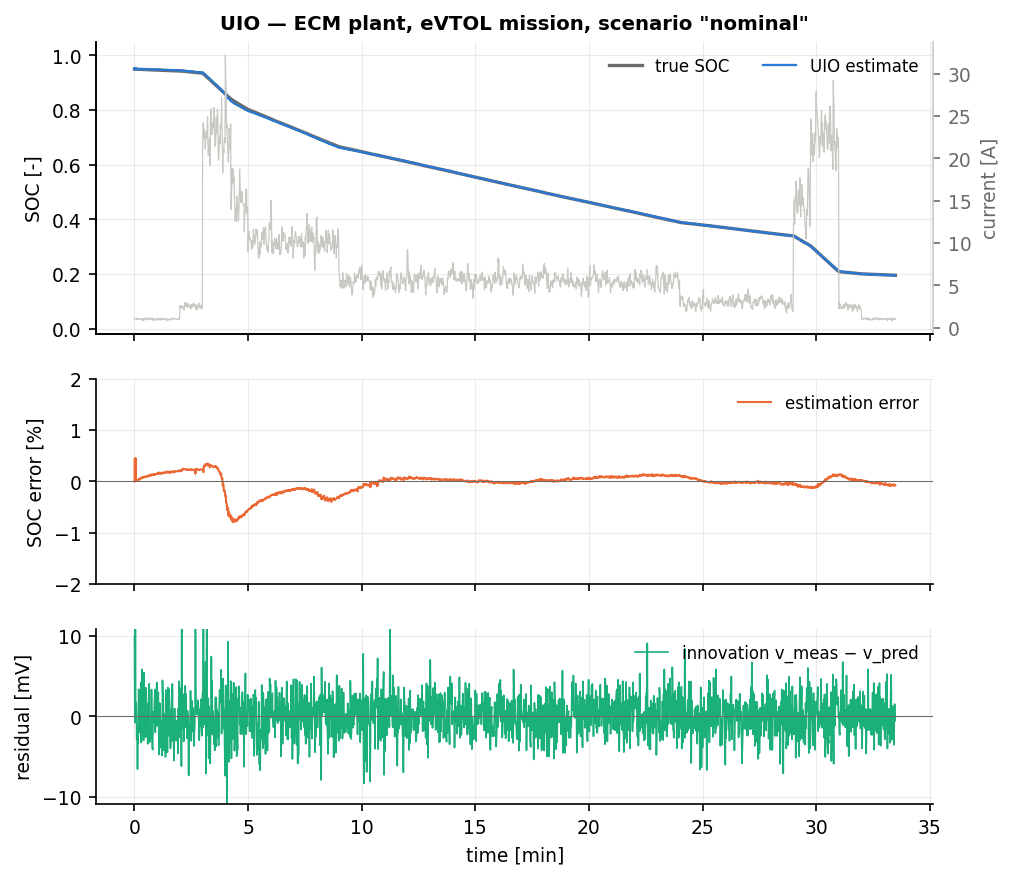
\includegraphics[width=\textwidth]{figures/cell_UIO_nominal.png}
\caption{UIO on the nominal eVTOL mission: true and estimated SOC (top), estimation error with the $\pm 2\sigma$ band when available (middle), voltage residual (bottom).}
\end{figure}
\begin{figure}[H]\centering
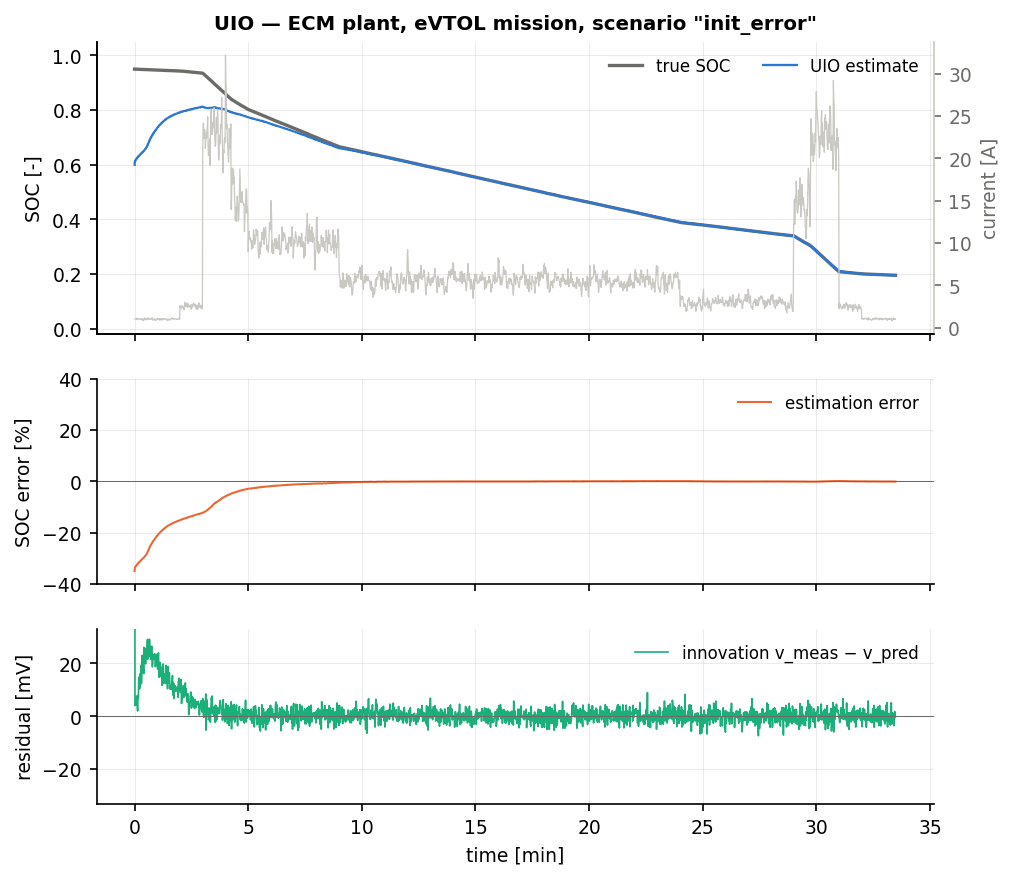
\includegraphics[width=\textwidth]{figures/cell_UIO_init_error.png}
\caption{UIO with a 35\,\% initial SOC error.}
\end{figure}

All numbers are over three seeds.  The UIO produces the most accurate steady-state SOC estimate
of any pure state observer in this family.  On \texttt{nominal} it reaches
$\mathrm{rmse}_{ss} = 0.0007$ against the EKF's $0.0005$; on \texttt{cold} $0.0018$ against the
EKF's $0.0016$; on \texttt{sensor\_dropout} $0.0006$ against $0.0046$ --- a factor of eight.  The
reason is that the decoupling removes the dominant error source of this plant, namely the fact
that the estimator's current is never quite the cell's current: even in the nominal scenario the
sensor carries an offset, a gain error, noise and quantisation, and an observer that is
structurally insensitive to all of it starts from a better place than one that treats it as
process noise.

On its target scenario the improvement is clear: \texttt{current\_bias} gives
$\mathrm{rmse}_{ss} = 0.0071$ against the Luenberger observer's $0.0085$ and the EKF's $0.0061$,
with a maximum error of $0.010$ against the Luenberger's $0.018$.  It is also the best observer
here on \texttt{aged\_cell} ($0.0190$), \texttt{param\_mismatch} ($0.0137$), \texttt{preisach}
($0.0088$) and \texttt{combined} ($0.0180$), which is a bonus rather than a design goal: a
capacity error acts partly like a current error and is partly decoupled with it.

The cost is exactly where \Cref{sec:uio-zeros} says it is.  On \texttt{init\_error} the UIO needs
$353$\,s to converge and on \texttt{combined} $1372$\,s --- the slowest in the family.  The fixed
mode at $|z|=0.99973$ ($\tau = 375$\,s) sets that timescale and no tuning changes it:
$0.35\,\mathrm{SOC}\times e^{-t/375}<0.02$ requires $t>1075$\,s.  A practical system would
therefore initialise the UIO from a rested OCV measurement, or run it in parallel with a fast
observer during start-up.

\subsection*{The single-particle plant, and why the degradation logic exists}
The SPM columns are where this chapter earns its \Cref{sec:uio-cond}.  With exact decoupling
($\theta\equiv1$) the UIO is by a wide margin the \emph{worst} estimator in the family on that
plant --- $\mathrm{rmse}_{ss}$ of $0.213$ on \texttt{nominal}, $0.598$ on \texttt{hot} and
$0.126$ on \texttt{current\_bias}, against $0.005$--$0.010$ for everything else --- and the cause
is entirely \eqref{eq:uio-cond}: $\norm{\mH}_\infty$ rises from $2.1$ to $15$--$21$ and the
structured ECM-versus-SPM voltage error is amplified with it.  The reconstructed ``current bias''
reaches $66$--$71$\,A, which is the observer stating in plain numbers that its own modelling
assumption is false.

With the conditioning budget and the admissibility gate of \eqref{eq:uio-gate} in place, the same
registration is the \emph{best} observer in the family on that plant: $0.0046$ on
\texttt{nominal} (against the DOB's $0.0069$ and the certified LQE observer's $0.0061$), $0.0044$
on \texttt{current\_bias} (DOB $0.0097$), $0.0223$ on \texttt{cold} (DOB $0.0333$), $0.0095$ on
\texttt{hot} and $0.0093$ on \texttt{param\_mismatch}.  The ECM behaviour is untouched, because
there the gate never closes.  The lesson generalises beyond this observer: a structure whose
correctness depends on a modelling assumption should compute the quantity that falsifies the
assumption and degrade on it, rather than assume it and fail.  The UIO gets that quantity for
free in $\hat{d}$.

\section{Summary}
Use the unknown-input observer when a sensor error must be rejected \emph{exactly} rather than
estimated: it gives the best steady-state SOC accuracy in this study, beats the EKF by a factor
of eight on a stuck-voltage fault, and provides a free current-bias reconstruction for
diagnostics.  Check $\operatorname{rank}(\mC\bm{E}) = \operatorname{rank}(\bm{E})$ before anything
else, but do not stop there: check $\norm{\bm{E}}_\infty/|\mC\bm{E}|$, which is the gain from any
unmodelled \emph{output} error to the state estimate and which a rank test does not see.  Design
$\mK_1$ by LQE rather than pole placement because the decoupled pair is only detectable, account
for any direct feed-through of the unknown input into the output separately, and monitor the
reconstructed input against its physical bound so the decoupling can be backed off when the
matching assumption stops holding.  Do not use it alone when a fast start-up transient matters ---
the invariant zeros of $(\mA,\bm{E},\mC)$ impose a floor on convergence time that no gain can
lower.
